\section{tasks::create\-Master\-Dark Class Reference}
\label{classtasks_1_1createMasterDark}\index{tasks::createMasterDark@{tasks::createMasterDark}}
Inheritance diagram for tasks::create\-Master\-Dark::\begin{figure}[H]
\begin{center}
\leavevmode
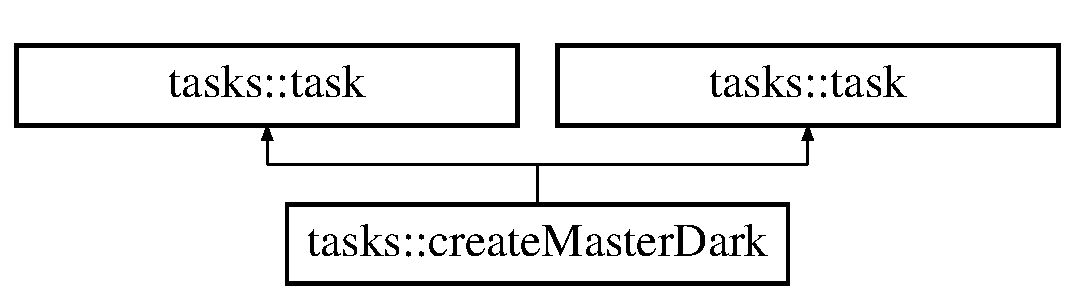
\includegraphics[height=2cm]{classtasks_1_1createMasterDark}
\end{center}
\end{figure}
\subsection*{Public Member Functions}
\begin{CompactItemize}
\item 
def \textbf{run}\label{classtasks_1_1createMasterDark_aaf59474fc1f553ecd05830b091eff02}

\item 
def \textbf{run}\label{classtasks_1_1createMasterDark_aaf59474fc1f553ecd05830b091eff02}

\end{CompactItemize}
\subsection*{Static Public Attributes}
\begin{CompactItemize}
\item 
string \textbf{name} = '{\bfcreate\-Master\-Dark}'\label{classtasks_1_1createMasterDark_6ae819dc4dc8afd8141b2fa2e298f639}

\item 
string \textbf{button\-Text} = 'Create Master DARK'\label{classtasks_1_1createMasterDark_673ea894f4c4df18ca8f7743a02d93fc}

\end{CompactItemize}


\subsection{Detailed Description}


\footnotesize\begin{verbatim}Create a master DARK from the dark file list
\end{verbatim}
\normalsize
 



The documentation for this class was generated from the following files:\begin{CompactItemize}
\item 
old/PANICtool-1.0/tasks.py\item 
old/tasks.py\end{CompactItemize}
